%!TEX root = ../aamas11storage.tex
%%%%%%%%%%%%%%%%%%%%%%%%%%%%%%%%%%%%%%%%%%%%%%%%%%%%
\section{Modular Battery Controller}\label{sec:introduction}
%%%%%%%%%%%%%%%%%%%%%%%%%%%%%%%%%%%%%%%%%%%%%%%%%%%%

Energy storage enables increasing levels of renewable energy in our electricity system, and the rapidly maturing supply chains for several battery technologies encourages electricity utilities, generators, and customers to consider using large battery systems. 

Consider the example scenario of a smart office building comprising of a set of loads (appliances in the building), some renewable sources (solar panels on the roof and a local wind turbine), and a modular battery system. The building is connected to the main grid, and economics govern that the grid power consumption of the building be maintained within the range $[0:p_h]$. Since there is little control over the demand in the building and certainly no control over the renewable generation, then for some period in the day it is possible that the power consumption of the building will fall outside this range. For instance, if the renewable generation is high relative to the building loads, then net consumption may fall below $0$. Similarly, if demand is higher than generation then the net building consumption may rise above $p_h$. In Figure \ref{fig:usecase} the Building Demand curve for the period prior to $t_1$ and after $t_2$, has this property. While this net demand is fixed for all practical purposes, we do have control over the use of the battery system. By suitably ordering the battery system to charge (act as a load) or discharge (act as a generator) at determined rates through this period we may influence the net demand in the building. Figure \ref{fig:usecase} shows how the appropriate battery response (Battery Charge) added to the net building consumption (Building Demand) ensures that the power drawn from the grid (Grid Supply) is maintained within the desired range.

\begin{figure}[ht]
\begin{center}
%!TEX root = ../aamas11storage.tex
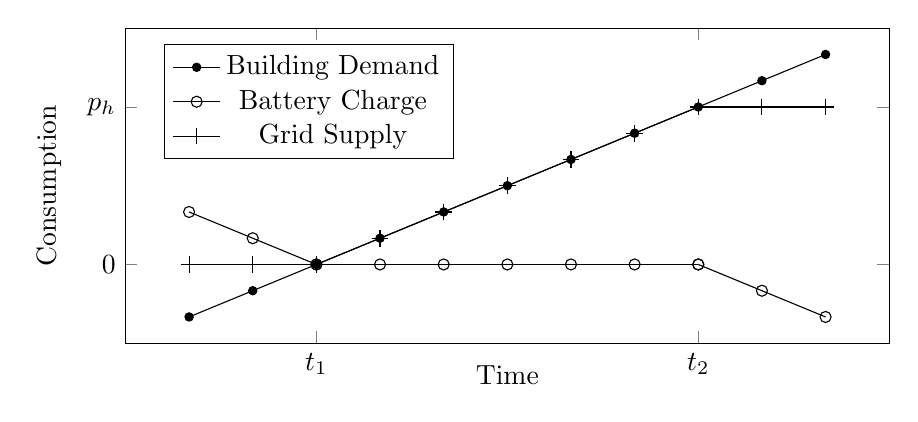
\begin{tikzpicture}

\begin{axis}[
width=0.8\columnwidth,height=4cm,scale only axis,
axis line style={-}, xtick style={-}, ytick style={-},
xlabel=Time,
ylabel=Consumption,
every axis y label/.style={at={(-0.1,0.5)},rotate=90,anchor=center}, 
every axis x label/.style={at={(0.5,-0.1)},anchor=center}, 
%grid=both, grid style={style=densely dotted},
xtick={2,8},
xticklabels={$t_1$,$t_2$},
ytick={0,6},
yticklabels={$0$,$p_h$},
legend style={at={(0.05,0.95)},anchor=north west}
] 

% Draw the Demand-Supply curve
\addplot[-,mark=*,mark size=1.5] expression[domain=0:10,samples=11] {x-2};
\addlegendentry{Building Demand} 

% Draw the Battery curve
\addplot[-,mark=o,mark size=2] expression[forget plot,domain=0:2,samples=3] {2-x}; 
\addplot[-,mark=o,mark size=2] expression[forget plot,domain=2:8,samples=7] {0}; 
\addplot[-,mark=o,mark size=2] expression[domain=8:10,samples=3] {8-x}; 
\addlegendentry{Battery Charge} 

% Draw the Grid supply curve
\addplot[-,mark=+,mark size=3] expression[forget plot,domain=0:2,samples=3] {0}; 
\addplot[-,mark=+,mark size=3] expression[forget plot,domain=2:8,samples=7] {x-2}; 
\addplot[-,mark=+,mark size=3] expression[domain=8:10,samples=3] {6}; 
\addlegendentry{Grid Supply} 
\end{axis} 
\end{tikzpicture} 

\end{center}
\caption{Use case scenario for a modular battery system.}
\label{fig:usecase}
\end{figure}

Large battery systems usually comprise of multiple modules and in many installations these may be controlled independently.  Modules may be operated in synchrony but often there are strategic reasons to keep some modules in a different state to others.  For example, if it is undesirable to change the direction of power flow between charging and discharging too frequently, a subset of modules may be used for each direction until it is necessary to change their roles.  Also, some technologies have specific requirements, such as the zinc-bromine flow battery for which a complete discharge at regular intervals is desirable to ``strip'' the zinc plating and ensure irregularities never have an opportunity to accumulate.  Where they exist these requirements place further constraints on module control.

Given, then, a requested rate of charging and discharging for a large battery installation, we would like a control algorithm for the set of component modules that implements the requested rate as the sum over the module rates of charging and discharging.  While hardwired control of such response is possible, it is not ideal since battery performance is susceptible to change over time and may diverge from normal. What is required is a means of adaptable control that accounts for such drift, and as such, a machine learning approach may be appropriate. 
%The input signal will be different every day but will have many features that are diurnal or nearly so, due to typical variations of electricity demand and solar and wind energy generation sources, and the repetitive patterns that may be seen over several days of the input signal suggest that a learning algorithm may be appropriate.  Our problem is to develop a method for on-line learning that will result in a useful control regime for a modular battery system, when installed at a new site and provided with an input signal derived from the electricity demand and renewable supply at that site.

\begin{figure*}[ht]
\begin{center}
%!TEX root = ../aamas11storage.tex
\begin{tikzpicture} [level distance=8.0em]
\tikzstyle{planbox}=[draw,text width=11.0em,rectangle split,rectangle split parts=3]
\tikzstyle{goalbox}=[draw,rounded corners=1.25em,minimum height=3em,minimum width=5em]

	
\tikzstyle{level 1}=[sibling distance=13.0em] 
\tikzstyle{level 2}=[level distance=7.0em] 

\node[goalbox,solid] {$G($r,k,s$)$}
	child {node[planbox] {$SetCharge$ 
			\nodepart{second} $\psi:satisfies(r,k,s,C),$\\$k>0$
			\nodepart{third} $set(k,C)$
		}
		child {node[goalbox] {$G($r,k-1,s'$)$}}
	}
	child {node[planbox] {$SetDischarge$ \nodepart{second}
			\nodepart{second} $\psi:satisfies(r,k,s,D),$\\$k>0$
			\nodepart{third} $set(k,D)$
		}
		child {node[goalbox] {$G($r,k-1,s'$)$}}
	}
	child {node[planbox] {$SetNotUsed$ \nodepart{second}
			\nodepart{second} $\psi:satisfies(r,k,s,N),$\\$k>0$
			\nodepart{third} $set(k,N)$
		}
		child {node[goalbox] {$G($r,k-1,s'$)$}}
	}
	child {node[planbox] {$Execute$ 
			\nodepart{second} $\psi:k==0$
			\nodepart{third} $operate()$ \\$evaluate()$
		}
	}
;

\end{tikzpicture}



\end{center}
\caption{Goal-plan hierarchy for the battery system with $k$ modules.}
\label{fig:gptree}
\end{figure*}


%%%%%%%%%%%%%%%%%%%%%%%%%%%%%%%%%%%%%%%%%%%%%%%%%%%%
\subsection{System Design}\label{subsec:design}
%%%%%%%%%%%%%%%%%%%%%%%%%%%%%%%%%%%%%%%%%%%%%%%%%%%%

Figure \ref{fig:gptree} shows a BDI controller for a battery system with $k$ modules. At the beginning of each period of deliberation, the environment posts the top-level goal $G(r,k,s)$. The controller responds by operating the battery system for that period in a suitable operational state that resolves the goal. Here $r$ specifies the desired response from the battery system and lies in the normalised range $[-1.0:+1.0]$ where $-1.0$ indicates a maximum discharge rate (where all modules are discharging) and $+1.0$ indicates a maximum charge rate (where all modules are charging). The parameter $s$ represents the current state of the battery system derived from sensor readings, and $k$ is initially set to the number of modules in the system. 

The resolution of the battery system decides how closely it can match the desired response and is determined by the number of modules $n$. For simplicity, we will assume homogeneous capacity of the modules (but with possibly different chemical properties and constraints), such that each module has a normalised capacity $c$ and $c*n=1.0$. Each module in turn may be configured in one of three states: charging (i.e $+c$), discharging (i.e. $-c$) or not in use (i.e. $0$). The sum of these values gives the net response of the system. By appropriately setting each module's operational state then, the response of the battery system may be adjusted in the range $[-1.0:+1.0]$ in steps of $\pm c$.

The BDI controller works by recursively setting the operational state of each module using the respective $Set*$ plans, and then finally executing the resulting configuration for one period using the $Execute$ plan. The {\em active execution trace} therefore always consists of the selection of $k$ high level $Set*$ plans followed by the selection of the $Execute$ leaf plan. 

The plans in the hierarchy are further explained below:

$SetCharge$: Set the configuration of module $k$ to {\em Charge} (i.e $+c$) for this period. The plan's context condition first checks that the internal constraints of module $k>0$ will not be violated by this operation. If the context condition fails then the plan is discarded, otherwise the configuration is updated and Goal $G$ reposted for module $k-1$.

$SetDischarge$: Set the configuration of module $k$ to {\em Discharge} (i.e $-c$) for this period. The plan's context condition first checks that the internal constraints of module $k>0$ will not be violated by this operation. If the context condition fails then the plan is discarded, otherwise the configuration is updated and Goal $G$ reposted for module $k-1$.

$SetNotUsed$: Set the operational state of module $k$ to {\em NotUsed} (i.e $0$). This means that the module will remain disconnected from use for this period. The plan's context condition first checks that the internal constraints of module $k>0$ will not be violated by this operation. If the context condition fails then the plan is discarded, otherwise the configuration is updated and Goal $G$ reposted for module $k-1$.

$Execute$: Leaf plan to physically operate the battery system. The plan executes only when $k=0$ which implies that all modules have been configured. The battery modules are then operated simultaneously for one period according to their assigned configurations. 

$Set*$ plans are discarded from consideration when their context condition does not hold for that period. For instance, plan $SetCharge$ may be discarded because module $k$ is only allowed to change charge directions once every four periods say, and charging it in this period will violate that constraint. Similarly, plan $SetDischarge$ may be discarded because the module may already be discharged and further discharge is not possible. 

Since such constraint checking is performed in the context condition of the plans prior to physical operation of the battery, then BDI failure recovery may be employed to select different $Set*$ plans until all internal constraints are satisfied. Note that failure recovery is not allowed for the $Execute$ plan because it runs for a full period and that is the limit for the decision making. In other words, only one try (in terms of physically operating the battery) is allowed per period.

Finally, the context condition of the $Set*$ plans performs {\em operational constraint checking} to decide if the configuration is admissible for module $k$: given the desired response $r$, the modules configured to so far i.e $[0 \ldots k-1]$, and the number of modules yet to be configured i.e $[k+1 \ldots n]$. For instance, a request of $+1.0$ is only serviceable when all modules are configured to charge. So, if module $k$ were to not charge (it may already be fully charged so further charging is not possible), then the operational constraint for module $k+1$ will fail because the ``bad'' configuration of module $k$ implies that regardless of how the remaining modules are configured, the response is bound to fall short of the request. When this happens, BDI failure recovery allows us to backtrack up the chain of active $Set*$ plans and choose a different path until all constraints are met. As such, the $Execute$ plan is run only with configurations that are functionally correct.



%%%%%%%%%%%%%%%%%%%%%%%%%%%%%%%%%%%%%%%%%%%%%%%%%%%%
\subsection{Programming for Adaptability}\label{subsec:constraints}
%%%%%%%%%%%%%%%%%%%%%%%%%%%%%%%%%%%%%%%%%%%%%%%%%%%%

The controller described so far is ideal, and if deployed will work perfectly for the initial specification of the system. However, if the physical battery properties were to change over time, then inevitably the system will perform sub-optimally. As an example, consider a time in the future where the  physical capacity of a module has deteriorated, so in effect it holds less charge than it did initially. Here, it is easy to see that some solutions that worked initially will no longer work. This is because the controller will not know where this new variable ``limit'' is, and will try charging the module in some situations only to find that the net battery response no longer matches the expected result. What we would like then, is to program the controller with adaptability in mind in order to rectify for some foreseeable changes.

In some way, we want to start with an ``ideal'' solution set, but allow modifications to it based on future changes in the environment. Preferably, the program should cater for inclusions to and deletions from this set over time, however for simplicity we will only consider deletions in this application. That is to say that we will program our controller with an ideal solution set based on initial specifications, and will allow for future changes that result in solution sets that are subsets of this. For our purpose this is acceptable since we generally expect batteries to perform ``less'' than ideal over time.

Our strategy for encoding such adaptability is using the BDI learning framework described in Section \ref{sec:framework}. To do this we add a feedback step that evaluates the actual battery response against the request for the purpose of learning. This is done in the $evalaute()$ step of the $Execute$ plan as shown in Figure \ref{fig:gptree}. The battery response is deemed successful only if it was within tolerance of the desired response, otherwise it is deemed failed.\footnote{Functionally the $Execute$ plan always succeeds as described in the system design, even though the evaluation against the goal for learning purposes may differ.} So every time the $Execute$ plan is invoked, the {\em evaluated} pass/fail result is recorded in the chain of active plans that led to that invocation. By training over the outcomes of plan selections in each situation, the system over time learns correct plan selection at each recursive level for the set of possible top-level requests. 

Note that useful learning takes place even while the system is performing ideally i.e. never experiences a failure. This is because ``internal'' failures during deliberation, when bad configuration paths are abandoned for alternatives, provide the necessary negative samples to build a useful classifier. The result is that the system works ideally while all the time collecting samples and building an incrementally better classifier for the state space experienced so far. Then, when the environment does finally change, it does not have to start learning from scratch and is better equipped to recover from the change than without.

Finally, the system only learns a response to the immediate request. It does not learn any temporal relationship in the sequence of top level goals. For instance, the request sequence may have some diurnal or seasonal pattern, however the proposed system does not attempt to learn this. This is acceptable since the time-scale for decision making (normally in the order of seconds) is very short compared to the frequency of any potential pattern.




%%%%%%%%%%%%%%%%%%%%%%%%%%%%%%%%%%%%%%%%%%%%%%%%%%%%
\subsection{Experimental Setup}\label{subsec:setup}
%%%%%%%%%%%%%%%%%%%%%%%%%%%%%%%%%%%%%%%%%%%%%%%%%%%%

We conduct experiments for a battery system with {\em five} modules. In this system, the charge state of each module is described by a discrete value in the range $[0:3]$ where zero indicates a fully discharged state and three indicates a fully charged state. As well as this, each module has an assigned configuration for the period from the set $\{+c, 0, -c\}$ where $c=1/n$ i.e $1/5$. The desired response is in the range $[-1.0:+1.0]$ in discrete intervals of $\pm c$ giving a total of $11$ possible requests. The full state space for the problem is given by $5 \cdot 11 \cdot 4^5 \cdot 3^5 \approx 13.7$ million. This is significant, however note that we do not have to learn over the entire state space since the filtering of nonsensical configurations by the plans context conditions reduces the space dramatically.

At the beginning of a learning episode the configuration of each module is reset to $0$. The charge state of each module, however, is left untouched and carries over from the previous episode as would be the case in the real system. This has some implications for the learning, particularly that the state space is not uniformly sampled while learning. Each episode corresponds to a single request from the environment. For simplicity of analysis, the environment only generates satisfiable requests given the state of the battery, such that a solution always exists for the generated request. The outcome of each episode is either no response (no configuration was chosen), or a single invocation of the $Execute$ plan that operates the battery and evaluates the response. The operational model is simple, so that charging adds $+c$ while discharging adds $-c$ to a module's charge state, otherwise the state is unchanged for the period i.e there is no charge loss. The tolerance level is set to $0.0$ so that the battery response is deemed successful only when the sum of the module configurations matches the request exactly.

The applicability threshold for plan selection is set to $40\%$ so plans with a likelihood of success below this value are discarded from the applicable set. The parameters for stability calculation are set to $k=1$ and $e=0.5$. For the stability-confidence measure, the averaging window uses the last five recordings while the weighting factor is $0.5$. Finally, each experiment is run five times and the reported results are averages from these runs.

\subsubsection{Experiment One}

In this experiment we model a scenario where battery module capacities deteriorate..

\begin{figure}[ht]
\begin{center}
%!TEX root = ../ijcai11storage.tex
\begin{tikzpicture}

\begin{axis}[
width=0.28\columnwidth,height=3cm,scale only axis,
axis line style={-}, xtick style={-}, ytick style={-},
%xlabel=Episodes,
%ylabel=Success,
every axis y label/.style={at={(-0.12,0.5)},rotate=90,anchor=center}, 
%every axis x label/.style={at={(0.5,-0.15)},anchor=center},
grid=both,grid style={-,style=densely dotted},
legend style={at={(0.5,0.25)},anchor=north west}
] 

\addplot[-] file {./data/storage1b.CF.tikzdata};
%\addlegendentry{Data} 

\end{axis} 
\end{tikzpicture} 

\end{center}
\caption{Controller performance with module capacity deterioration.}
\label{fig:experiment1}
\end{figure}

\subsubsection{Experiment Two}

In this experiment we model a scenario where some modules malfunction..

\begin{figure}[ht]
\begin{center}
%!TEX root = ../ijcai11storage.tex
\begin{tikzpicture}

\begin{axis}[
width=0.5\columnwidth,height=4cm,scale only axis,
axis line style={-}, xtick style={-}, ytick style={-},
%xlabel=Episodes,
%ylabel=Success,
every axis y label/.style={-,at={(-0.12,0.5)},rotate=90,anchor=center}, 
%every axis x label/.style={at={(0.5,-0.15)},anchor=center},
grid=both,grid style={-,style=densely dotted},
legend style={at={(0.5,0.25)},anchor=north west}
] 

\addplot[-] file {./data/storage2b.CF.tikzdata};
%\addlegendentry{Data} 

\end{axis} 
\end{tikzpicture} 

\end{center}
\caption{Controller performance with multiple module malfunctions over time.}
\label{fig:experiment2}
\end{figure}

\subsubsection{Experiment Three}

In this experiment we model a scenario where the controller must re-learn.

\begin{figure}[ht]
\begin{center}
%!TEX root = ../aamas11storage.tex
\begin{tikzpicture}

\begin{axis}[
width=0.8\columnwidth,height=4cm,scale only axis,
axis line style={-}, xtick style={-}, ytick style={-},
xlabel=Episodes,
ylabel=Success,
every axis y label/.style={-,at={(-0.12,0.5)},rotate=90,anchor=center}, 
%every axis x label/.style={at={(0.5,-0.15)},anchor=center},
grid=both,grid style={-,style=densely dotted},
legend style={at={(0.5,0.25)},anchor=north west}
] 

\addplot[-] file {./data/storage3mb.CF.tikzdata};
%\addlegendentry{Data} 

\end{axis} 
\end{tikzpicture} 

\end{center}
\caption{Controller performance when previous learning must be overcome.}
\label{fig:experiment3}
\end{figure}



%%%%%%%%%%%%%%%%%%%%%%%%%%%%%%%%%%%%%%%%%%%%%%%%%%%%
\subsection{Analysis}\label{subsec:analysis}
%%%%%%%%%%%%%%%%%%%%%%%%%%%%%%%%%%%%%%%%%%%%%%%%%%%%

Impact of applicability threshold: Reduces number of Execute tries by $12\%$ that is substantial when considering battery life. The difference in performance with and without the applicability threshold is not significant.\footnote{Source: Repository revision 475. Number of calls to $Execute$ averaged over five runs was $40000$ for test storage2 and $35203$ for test storage2b giving a saving of $12\%$.}

Impact of data filtering: Reduces the training set size by an average of $74\%$ across all plans over all repeats of the experiment. The difference in performance with and without data filtering is not significant.\footnote{Source: Repository revision 475. The average training set size for all plans over five runs was $56590.2$ for test storage2 and $14708.8$ for test storage2m giving a saving of $74\%$.}

%The system is (purposely) similar in design to the Towers of Hanoi problem of \cite{Singh:RAS10}. In some respects, it is simpler because the solutions are always at recursive depth $k$. Moreover, the non-leaf $Set*$ plans do not have side-effects when they fail and leave the initial state unaltered. Finally, a solution always consists of a single $Execute$ action whereas in the Hanoi problem it consists of possibly several $Move$ actions\footnote{One point of difference is that this is not a universal library where a solution can always be found. For some requests, no solution will be possible given the internal state of the modules.}.

%Nonetheless, the problem captures a real world problem where it is not straightforward to hand-craft a functional hierarchy and where learning is justified. We do not have a solution to begin with. Then, the size of the problem is still significant - the flow battery in CSIRO Newcastle has $10$ internal modules, so with three possible module states that represents $3^{10}=59049$ possible configurations for a given request. Finally, it offers a realistic scenario for re-learning a solution due to significant changes in the environment. For instance, if an internal module were to fail and had to be replaced, then prior learning may no longer work effectively, and the system will have to adjust and re-learn it's response based on the new characteristics of the updated module.
